\documentclass[12pt]{article}

% margins and page style
\usepackage[margin=2.5cm]{geometry}
\usepackage{fancyhdr}
\pagestyle{fancy} 

% spaces between paragraphs
\usepackage[parfill]{parskip}

% fonts
\usepackage[T1]{fontenc}
\usepackage[scaled=0.92]{helvet}
\renewcommand*\familydefault{\sfdefault}

% font size of section headings
\usepackage{sectsty}
\sectionfont{\fontsize{14}{15}\selectfont}

% tables 
\usepackage{booktabs}
\renewcommand{\arraystretch}{1.5}

% figures
\usepackage{graphicx}
\usepackage[font=small,labelfont=bf]{caption} 

% colors
\usepackage[dvipsnames,svgnames,hyperref,table]{xcolor}

% hyperlinks
\usepackage{hyperref}
\hypersetup{
  pdfauthor={Erin C. McKiernan},
  colorlinks=true,
  urlcolor=Bittersweet,
  linkcolor=blue,
  citecolor=Purple,
}

% bib options
\let\oldbibliography\thebibliography
\renewcommand{\thebibliography}[1]{\oldbibliography{#1}
\setlength{\itemsep}{0pt}} 
\usepackage[numbers,sort&compress]{natbib} 
\bibliographystyle{unsrtnat}

% title and authors
\usepackage{authblk}
\title{\vspace{-1.8cm}\Large{\textbf{Electromyography: recording the
      electrical activity of skeletal muscles in the body's lever
      systems}}}
\author[1]{Erin C. McKiernan}
\affil[1]{\small{Departamento de F\'isica, Facultad de Ciencias, Universidad Nacional Aut\'onoma de M\'exico}}

\date{}

%%%%%%%%%%%%%%%%%%%%%%%%%%%%%%%%%%%%%%%%%%%%%%%%%%%%%%%%%%%%
 
\begin{document}
\maketitle

\section*{OVERVIEW}
In this laboratory practical, students will learn about the basics of muscle structure and function, and how muscles provide the force to move the three types of lever system found in the human body. Students will learn how to record from their skeletal muscles using electromyography, recording muscles from all three types of lever system. Overall, this practical will help students understand the biomechanics of the musculoskeletal system, and how movement is related to electrical activity in excitable muscle cells.

\section*{SPECIFICATIONS}
\begin{tabular}{p{6cm} p{10cm}}
\textbf{Level of study:} & Undergraduate \\
\textbf{Degree programs:} & Biology, Physics, Biomedical Physics, others \\
\textbf{Semester:} & 4th (i.e. 2nd year undergrads) \\ 
\textbf{For use in courses:} & Systems Physiology, others \\
\textbf{Recommended prior courses:} & Molecular \& Cellular Biology \\
\textbf{Duration of practical:} & 1-2 hours \\
\textbf{Setting:} & Classroom or laboratory \\
\textbf{Safety considerations:} & None \\
\textbf{Other indications:} & Wear loose clothing to permit electrode placement
\end{tabular}

\section*{OBJECTIVES}
\textbf{Before doing this lab you should be able to:}
\begin{itemize}
\item identify and describe the function of different cellular organelles and compartments
\item understand the basics of action potential generation at the neuromuscular junction 
\item understand basic concepts in physics, like work and force 
\end{itemize}
 
\vspace{0.3cm}

\textbf{In this lab you will:}
\begin{itemize}
\item learn how to record electromyograms (EMGs) from skeletal muscles
\item observe and record changes in the EMG when muscles contract and relax
\item investigate the effects of changing the speed and force of contraction on EMG signals
\item compare and contrast recordings from three different lever systems in the body
\end{itemize}

\vspace{0.3cm}
 
\textbf{After doing this lab you should be able to:}
\begin{itemize}
\item explain the relationship between muscle cell electrical activity and muscle contraction
\item understand the basics of EMG recording
\item design further experiments to investigate the activity of different skeletal muscles
\end{itemize}

\section*{EQUIPMENT}

 \begin{itemize}
	\item Muscle SpikerBox (Backyard Brains)
    \item 3 surface electrodes (Backyard Brains or other provider)
    \item orange cable with alligator clips to connect electrodes to SpikerBox (Backyard Brains)
    \item cable to connect SpikerBox to a computer, tablet, or smartphone (Backyard Brains)
 	\item computer or smartphone with free Backyard Brains SpikeRecorder software installed
\end{itemize}

\section*{BACKGROUND}

\subsection*{Skeletal muscles provide force to move levers in human body}

Movements of the human musculoskeletal system are accomplished by sets of bones, joints, and muscles that work together much like lever systems \cite{leversOLI,openStax2016lever}. A lever is composed of a rigid rod or bar (the lever arm) that pivots about a fixed point (the fulcrum) and can move a load or overcome a resistance when a force is applied. Levers are grouped into three classes, depending on the relative placement of the fulcrum, force applied, and the load or resistance (Fig. \ref{fig:levers}). Class 1 levers have a central fulcrum with the force applied on one side and the load on the other (e.g., a crowbar). For class 2 levers, the load is central and the force and fulcrum are on either side (e.g., a wheelbarrow). For class 3 levers, the force is applied centrally and the fulcrum and load on are opposing ends of the arm (e.g. a pair of tweezers is a pair of 3rd class levers). 

\begin{figure}[h!]
\centering
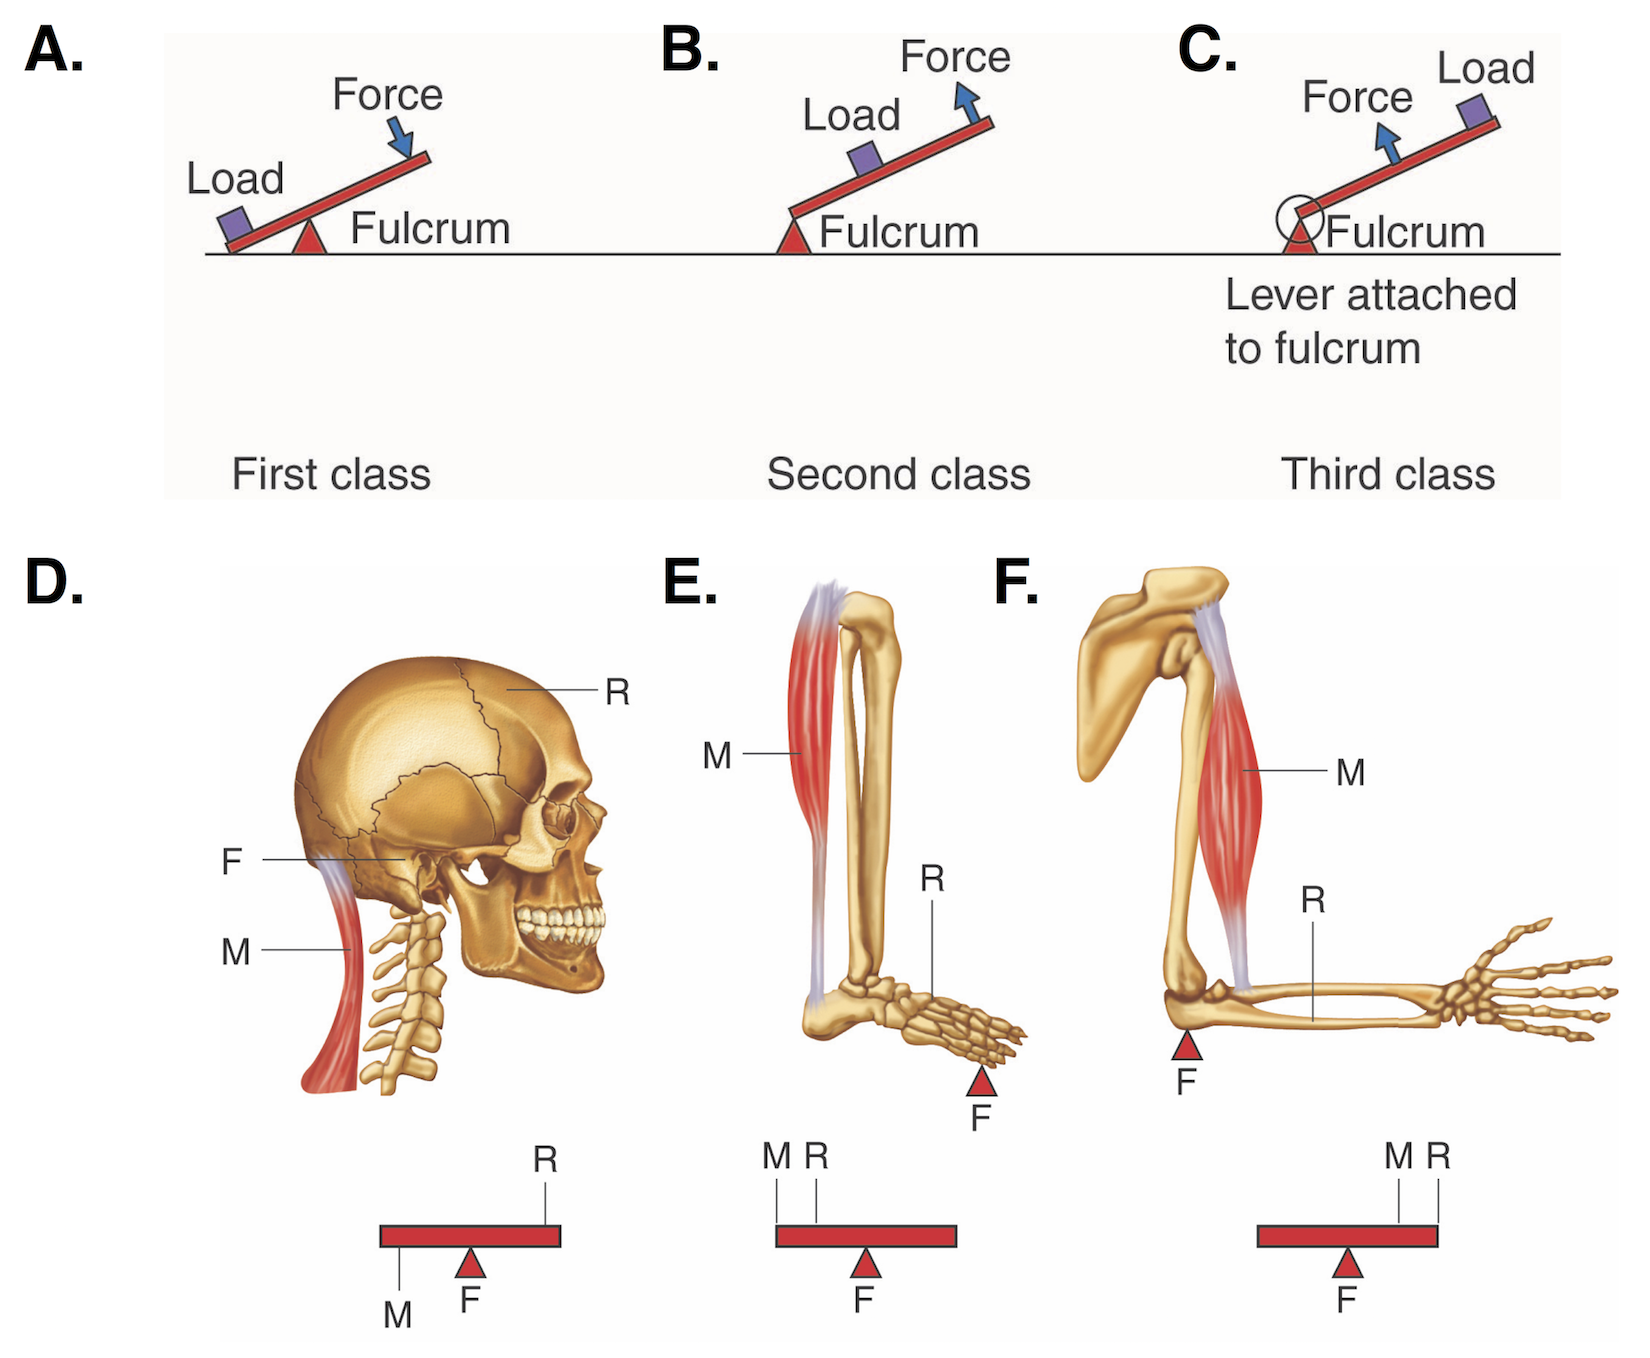
\includegraphics[width=0.9\textwidth]{figures/levers2.png}
\caption{The three classes of levers (A-C.) and examples in the human body (D-F.). M - muscle, F - fulcrum, and R - resistance. Image: Open Learning Initiative \cite{leversOLI}, CC BY.}
\label{fig:levers}
\end{figure}

In the human body, bones act as lever arms and joints as fulcrums. The force to overcome a resistance or lift a load is provided by the contraction of skeletal muscles, which are attached to the bones by tendons \cite{leversOLI,openStax2016lever}. All three classes of levers are found in the human body, though some are more common than others \cite{leversOLI}. Class 1 levers are rare, but a few examples do exist, including the bone-joint system responsible for head flexion and extension (lowering or lifting the head, respectively; Fig. \ref{fig:levers}D). In this case, the fulcrum is the joint between the cranium and the first cervical vertebrae. The load, or resistance, is the weight of the head itself. The force to lift the head is applied by contraction of skeletal muscles in the neck and upper back, including the splenius capitis and semispinalis capitis \cite{openStax2016axial}.  The lever arm in this case is not as obvious as in long-bone systems, but is the cranium itself. A line can be imagined running diagonally from the neck muscles on the left, up through the cervical joint, and ending at a point on the cranium above the eye socket.

When a person stands on tip toes, we can see an example of a class 2 lever in the human body (Fig. \ref{fig:levers}E) \cite{leversOLI}. The foot is the lever arm, the joints between the bones of the foot and those of the toes (the metatarsophalangeal joints) act as the fulcrum, and the load is the person's body weight. The force required to lift the body is provided by contraction of the gastrocnemius and soleus muscles in the back of the leg.

Class 3 levers are the most common type found in the human body \cite{leversOLI}. The classical example is the complex formed by the biceps brachii, elbow, and forearm. In this example, the forearm is the lever arm, the elbow joint is the fulcrum, and the force required to move the arm upwards (flex) or lift a load is provided by the bicep.

\subsection*{Skeletal muscle structure}

To understand how muscles contract, we must first know about their structure. Skeletal muscles are composed of multiple fascicles, which are bundles are many smaller muscle fibers surrounded by a layer of connective tissue (the perimysium) \cite{openStax2016muscle}. In many skeletal muscles, the fascicles are aligned parallel to one another, running along the length of the muscle \cite{openStax2016lever}. Other muscles show a circular fascicle arrangement. Some muscles have fascicles which meet at one attachment point (convergent), while others feather out from a central tendon (pennate). The arrangement of the fascicles affects the direction and angle at which the fibers can pull, and also affects force generation in the muscle \cite{openStax2016lever}.

Each muscle fiber is itself composed of many smaller myofibrils, containing the molecular machinery for contraction \cite{openStax2016muscle}. Surrounding the muscle fiber is the plasma membrane, or sarcolemma. In the sarcolemma are embedded transmembrane proteins, like ion channels that mediate currents and permit the generation of muscle action potentials (APs) \cite{openStax2016muscle}. These APs propagate via invaginations in the sarcolemma, known as tranverse (T) tubules (Fig. \ref{fig:ttubules}). Positioned right next to the T-tubules is the sarcoplasmic reticulum, the equivalent of endoplasmic reticulum in muscle. Here, select channels respond to the changes in voltage generated by the propagating APs to initiate intracellular events that activate the contractile machinery \cite{openStax2016muscle}.

\begin{figure}[h]
\centering
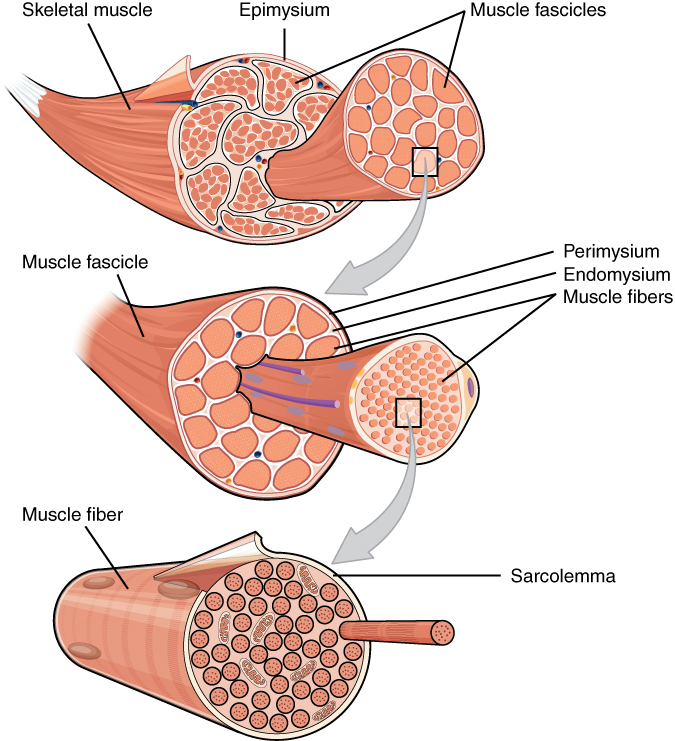
\includegraphics[width=0.7\textwidth]{figures/muscleStructure.jpg}
\caption{Muscle structure and levels of organization. Top: whole
  muscle showing fascicles. Middle: single fascicle showing muscle
  fibers.  Bottom: single muscle fibers showing myofibrils. Image:
  OpenStax \cite{openStax2016muscle}, CC BY.}
\label{fig:fibers}
\end{figure}

The functional contractile unit of skeletal muscle is known as the sarcomere \cite{openStax2016muscle}. In skeletal muscles, sarcomeres are arranged in series along the length of the myofibrils. Regular and repeated changes in the density of particular proteins in the sarcomeres is what give skeletal muscles their striped, or striated, appearance under a microscope.

\begin{figure}[h!]
\begin{minipage}{.45\textwidth}
\centering
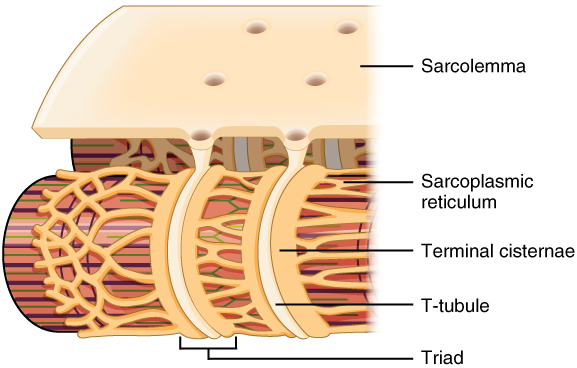
\includegraphics[width=0.95\textwidth]{figures/T-tubule.jpg}
\end{minipage}%
\begin{minipage}{.52\textwidth}
\centering
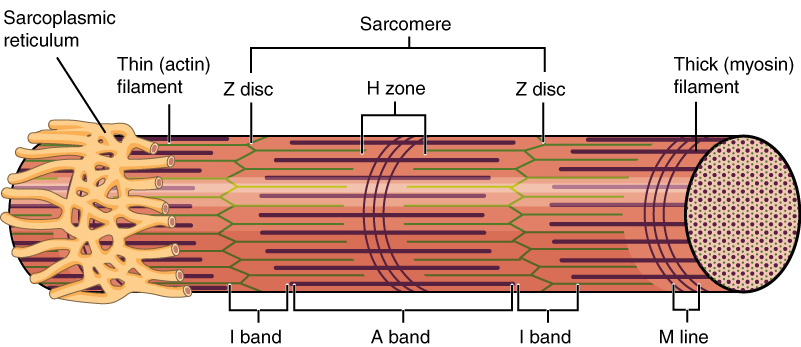
\includegraphics[width=0.95\textwidth]{figures/SRsarcomere.png}
\end{minipage}
\caption{\textit{Left}: Invaginations in the sarcolemma form the T-tubles, flanked by sarcoplasmic reticulum (SR). \textit{Right}: Near the SR, proteins are arranged in sarcomeres. Different zones are delineated within the sarcomere by the presence and overlap of select proteins and filaments. Image: OpenStax \cite{openStax2016muscle}, CC BY.}
\label{fig:ttubules}
\end{figure}

\subsection*{Sliding filament model and length-tension relationship}
Sarcomeres contain a number of proteins, like titin, which acts as a ``molecular spring'' and is important for establishing elasticity and passive tension in muscles \cite{granzier2006giant}. However, the basis for contraction lies in the interaction between actin (thin) filaments and myosin (thick) filaments \cite{openStax2016contraction}. These filaments are arranged in parallel, with areas of overlap. Myosin can attach to actin via binding sites in the myosin head region, forming what is called a cross-bridge. When the head moves, this causes the filaments to slide past one another, increasing the area of overlap and shortening the sarcomere.
When this happens in multiple sarcomeres along the length of the myofibril, the myofibril shortens. If the same effect occurs in many myofibrils within many fascicles, the entire muscle shortens and produces a contraction. This description of the interaction of the myosin and actin filaments is called the sliding filament model of contraction. The steps by which the myosin and actin filaments engage, slide, disengage, and then reset is collectively called the cross-bridge cycle \cite{openStax2016contraction} (discussed in more detail below).
  
\begin{figure}[h!]
\centering
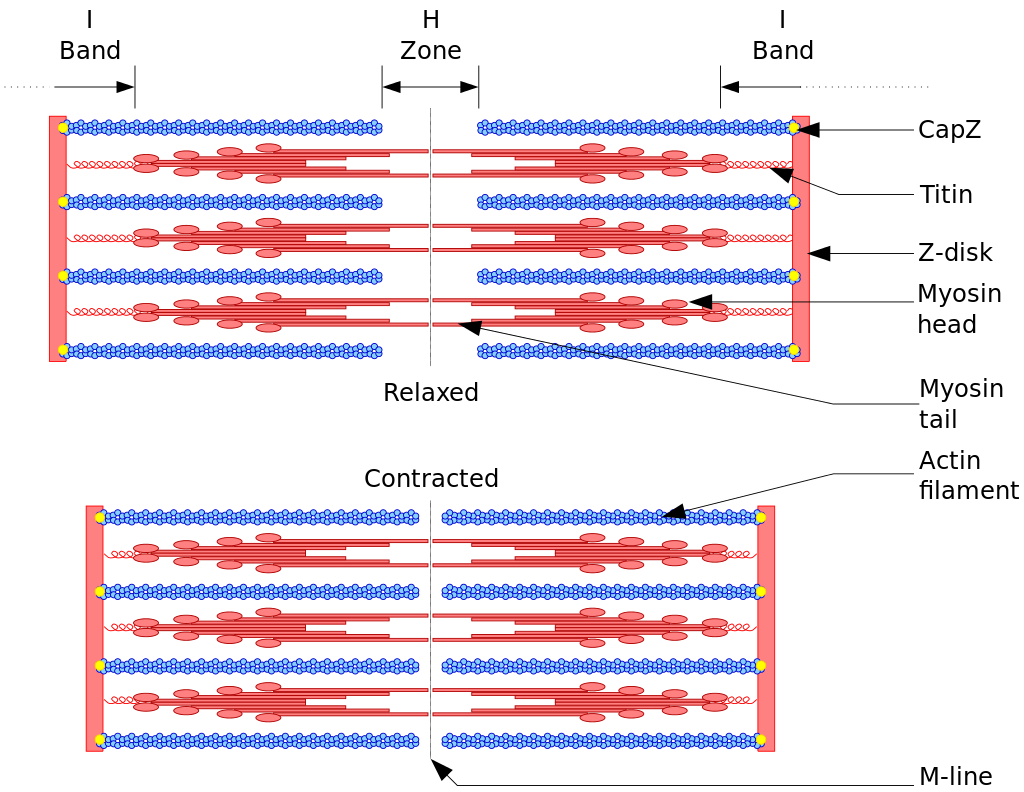
\includegraphics[width=0.8\textwidth]{figures/sarcomere.png}
\caption{Sliding filament model of muscle contraction. Top: sarcomere in relaxed muscle. Filaments have areas of overlap, but are not actively engaged. Bottom: sarcomere in contracted muscle. Myosin heads bind to actin filaments, move inward toward the M-line, and slide to shorten the sarcomere. Image: David Richfield \cite{richfieldSarcomere}, CC BY-SA.}
\label{fig:sarcomere}
\end{figure}

There is an optimal, intermediary level of filament overlap that produces maximal tension in the muscle \cite{openStax2016nervous}. Too little overlap and the filaments cannot bind and interact; too much overlap and there is no capacity for additional filament sliding. The relationship between filament overlap (i.e., the length of the sarcomere) and muscle tension is called the length-tension relationship, and is shown in Fig.\ref{fig:tension}.

\begin{figure}[h!]
\centering
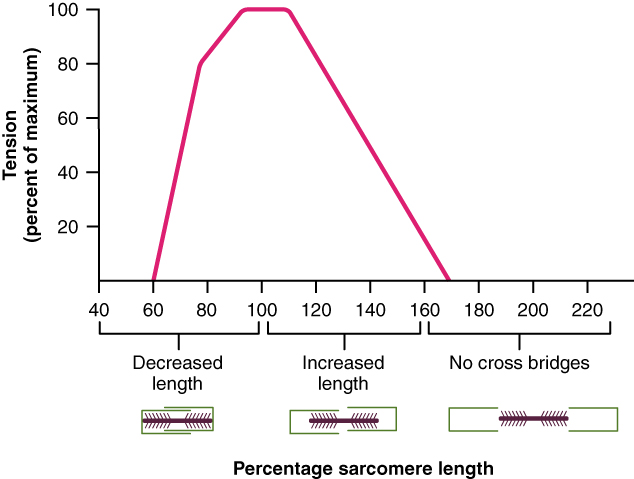
\includegraphics[width=0.75\textwidth]{figures/lengthTension.jpg}
\caption{Length-tension relationship in muscle. Maximal tension is produced when actin and myosin filaments have optimal overlap for sliding, i.e., at around 80-120\% of the sarcomere's resting length. Image: OpenStax \cite{openStax2016nervous}, CC BY}
\label{fig:tension}
\end{figure}

\subsection*{Excitation-contraction coupling and cross-bridge cycling}
How does an action potential (AP) generated at the neuromuscular junction (NMJ)\footnote{Action potential generation at the NMJ is not discussed herein, but can be reviewed in Ch. 7 of \cite{guyton2016book}.} lead to cross-bridge cycling within the sarcomeres? In other words, how is excitation coupled to contraction? The AP propagates from the NMJ down through the T-tubules to reach the interior of the myofibrils \cite{openStax2016contraction}. Within the T-tubule, the change in voltage activates a voltage-gated calcium channel known as Ca$_{v}$1.1, or the dihydropyridine receptor (DHPR) \cite{schneider2012skeletal}. The DHPR is mechanically linked to the ryanodine receptor (RyR) embedded in the membrane of the sarcoplasmic reticulum (SR). Activation of DHPR causes a conformational change that, in turn, activates RyR, opening the channel and allowing calcium to exit the SR down its electrochemical gradient \cite{schneider2012skeletal}. This increase in free intracellular calcium, in turn, permits cross-bridge formation. If calcium is not present, cross-bridges cannot form because a complex of tropomyosin and troponin proteins blocks the myosin binding site on the actin filaments. When calcium binds with troponin, it results in a conformational change that moves tropomyosin out of the way and allows myosin and actin to bind \cite{openStax2016contraction}. Once they are bound, the filaments can slide.

To continue cycling, the myosin and actin filaments must also be able to unbind and reset their position. This process requires the input of energy in the form of ATP \cite{openStax2016contraction}. When myosin binds with ATP, it detaches from actin. Subsequently, the ATP is hydrolyzed and the energy released is used to move the myosin head back into the ``cocked'' position, ready to bind with actin. ADP and one inorganic phosphate remain attached to the myosin head. Then, myosin binds to actin and releases the inorganic phosphate. Next, the myosin head releases the ADP and moves inward in what is called the power stroke, which causes the actin filaments to slide toward the midline and shorten the sarcomere. Cross-bridge cycling continues as long as sufficient ATP and calcium are present. The muscle relaxes when calcium is pumped back into the SR and is no longer available, thereby allowing tropomyosin to block the actin-myosin binding site once more \cite{openStax2016contraction}.

\textbf{Study question:} How do the molecular details of excitation-contraction coupling differ in cardiac and smooth muscle, compared to skeletal muscle?

\subsection*{Muscle fiber responses, summation, and recruitment}

The response of a muscle to stimulation depends on the timing and strength of the stimulus \cite{openStax2016nervous}. If only a brief stimulus occurs, then a muscle fiber will respond with a single AP and only a short (tens to hundreds of milliseconds) twitch will be produced. Because the intracellular events needed to produce a twitch take longer than those to generate an AP, another AP can arrive before the muscle fiber has fully relaxed. If this occurs, the second response will add to the tension already present in the muscle in a process called summation. Achieving sustained muscle fiber contraction and generating tension large enough to do work requires the summation of multiple stimulatory events. 

In addition to summation within single muscles fibers, multiple fibers are activated to achieve whole-muscle contraction. A motor neuron and all the muscle fibers it sends signals to (innervates) within a muscle is called a motor unit. Motor units can vary in size, with some motor neurons innervating few fibers (small unit) and others innervating many (large unit). 
Muscles can vary the force they generate depending on the number and type of motor units that are recruited.

\vspace{0.2cm}

\begin{figure}[h!]
\begin{minipage}{0.45\textwidth}
\centering
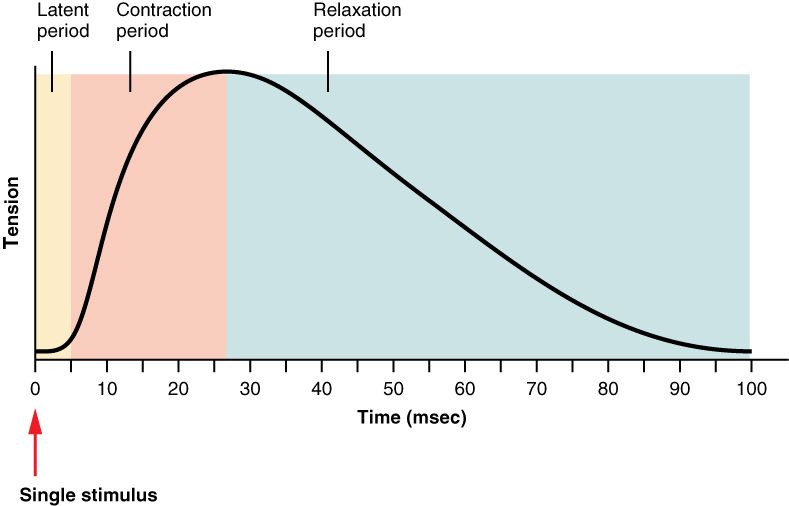
\includegraphics[width=0.95\textwidth]{figures/myogram.jpg}
\end{minipage}%
\begin{minipage}{0.55\textwidth}
\centering
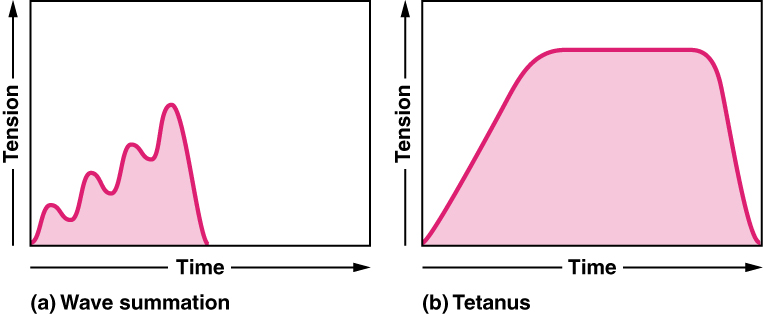
\includegraphics[width=0.95\textwidth]{figures/summation.jpg}
\end{minipage}
\caption{Muscle responses. \textit{Left:} Tension developed during a twitch resulting from a single, brief stimulus. \textit{Right:} Multiple stimuli  in quick succession produce summation and increasing tension. If stimulation frequency is high enough, the responses fuse into tetanus, achieving maximal tension and smooth contraction. Image: OpenStax \cite{openStax2016nervous}, CC BY.}
\label{fig:twitch}
\end{figure}

\subsection*{Measuring electrical activity of skeletal muscles - electromyogram}

To record the electrical activity of muscles we use a technique called electromyography, and the recordings we obtain are called electromyograms (EMGs) \cite{garcia2011surface}. EMG recording can be done invasively by inserting electrodes into the muscle of interest, or non-invasively by using surface electrodes placed on the skin above the muscle (Fig. \ref{fig:emg}). Electrode insertion has the advantage of giving `cleaner' EMG recordings in which the activity of separate motor units can be distinguished. However, electrode insertion can be painful and requires sterile conditions to prevent infection, making this type of recording not ideal for classroom settings. Surface electrodes, in contrast, can be easily applied to and removed from the skin without injury. The limitations of this type of extracellular recording include only being able to record from superficial muscles, and recordings which often do not allow for the separation of individual motor units \cite{garcia2011surface}. These limitations are not prohibitive and are typically outweighed by the benefits of non-invasiveness, but should be kept in mind when thinking about electrode placement and data analysis. 

One of the most common recording configurations is known as a bipolar EMG, or a single differential EMG \cite{garcia2011surface}. Two surface electrodes are placed on the skin above the muscle just a few centimeters apart (Fig. \ref{fig:emg}). By subtracting the signals recorded at the two points and then amplifying the difference, common signals that may result from muscles outside the recording site are largely excluded, and predominantly local changes in activity are recorded. This configuration thereby decreases muscle cross-talk \cite{garcia2011surface}. 

\begin{figure}[h!]
\centering
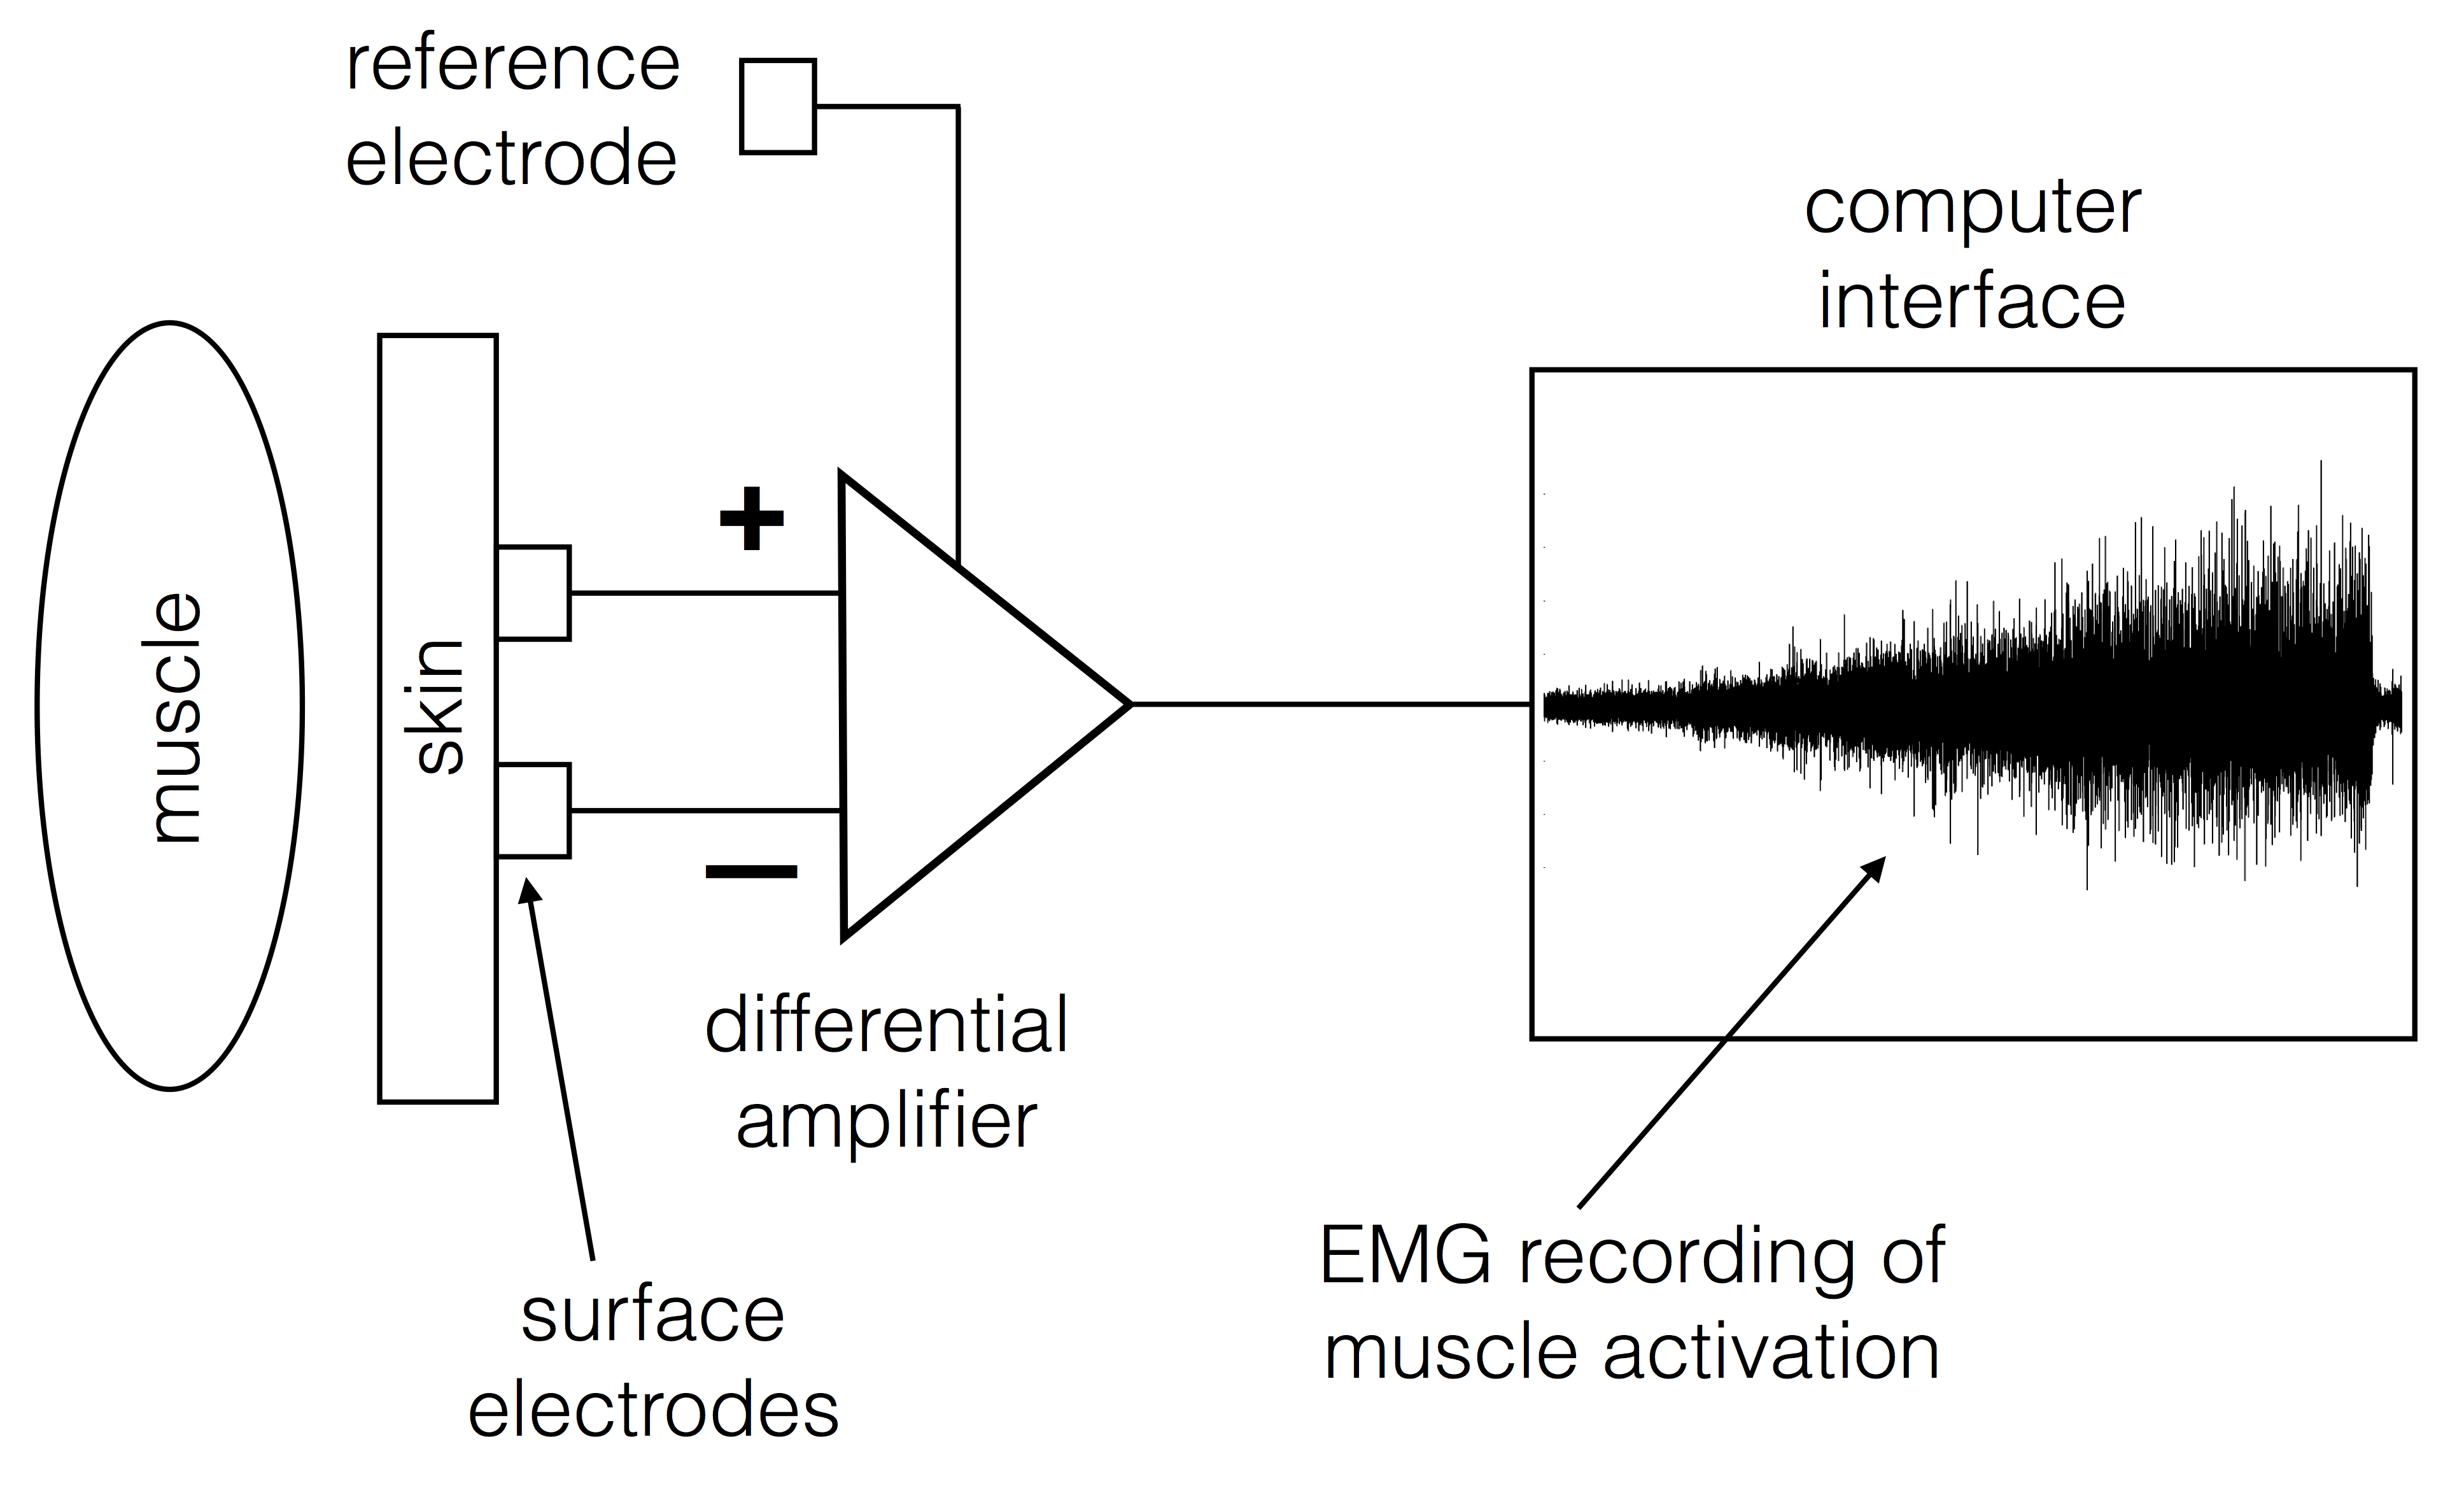
\includegraphics[width=0.7\textwidth]{figures/emgAmp.png}
\caption{Bipolar EMG recording setup. For simplicity, not all body or recording components are shown. Image credit: Erin C. McKiernan, CC BY}
\label{fig:emg}
\end{figure}

Bipolar surface EMGs can tell us several things about muscle activity \cite{garcia2011surface}. One is the timing of muscle activation and relaxation. Most muscles show very little activity at rest. When activated, we see a noticeable increase in the occurrence of electrical impulses, as shown in Fig. \ref{fig:emg} (right-hand side). When the muscle relaxes, these impulses disappear and we record only the baseline noise. The timing of muscle activity can then be correlated with other measures. We can also, to some extent, estimate the force or effort exerted during a contraction. As the subject increases the force of contraction, we see an increase in both the frequency of electrical impulses and the signal amplitude. These changes result from two factors: (1) a higher frequency of firing in already active motor units, and (2) the recruitment of additional motor units. Remember, we are recording the activity of multiple motor units. With increasing contraction force, more motor units are recruited and begin to fire, their activity sums, and contributes to the frequency and amplitude increases.

\subsection*{Study questions} 
\begin{enumerate}
\item Where will you need to place the electrodes to record EMGs from a class 1, class 2, or class 3 lever system?
\item Will you be able to record from any muscle you want in each lever system? Why, or why not? 
\item How will you know if you have correctly placed the electrodes?
\end{enumerate}

\section*{PROCEDURE}

Before beginning, make sure you have all the necessary equipment and have installed the Backyard Brains recording software on your computer or smartphone. The following steps will guide you in setting up the equipment and carrying out recordings.

\subsection*{1. Setup EMG recordings}

The Backyard Brains Muscle SpikerBox comes fully assembled and ready to record. All you have to do is connect the battery, cables, and electrodes.

\vspace{0.2cm}

\begin{enumerate}
\item Connect the 9V battery to its terminals on the Muscle SpikerBox
\item Connect the black/blue or green cable to the corresponding computer or smartphone port on the Muscle SpikerBox; note that the smartphone cable is directional, make sure you have the correct end inserted into the device
\item Connect the other end of the black/blue or green cable to your computer or smartphone
\item Connect the orange cable to its corresponding port on the Muscle SpikerBox
\item Place the surface electrodes over the muscle of interest, just a few centimeters apart and oriented parallel to the muscle fibers; remember, to record each lever type, you will have to change the electrode placement between experiments
\begin{itemize}
\item Class 1 lever - example muscle of interest: splenius capitis
\item Class 2 lever - example muscle of interest: gastrocnemius
\item Class 3 lever - example muscle of interest: biceps brachii
\end{itemize}
\item Connect each of the red aligator clips on the end of the orange cable to one of the surface electrodes; make sure the metal clips do not touch and try to avoid entangling the cables 
\item Hold the black aligator clip (reference) in your hand, or connect it to another surface electrode on the back of your hand or some other area away from the recording site

\vspace{0.2cm}

\begin{figure}[h!]
\centering
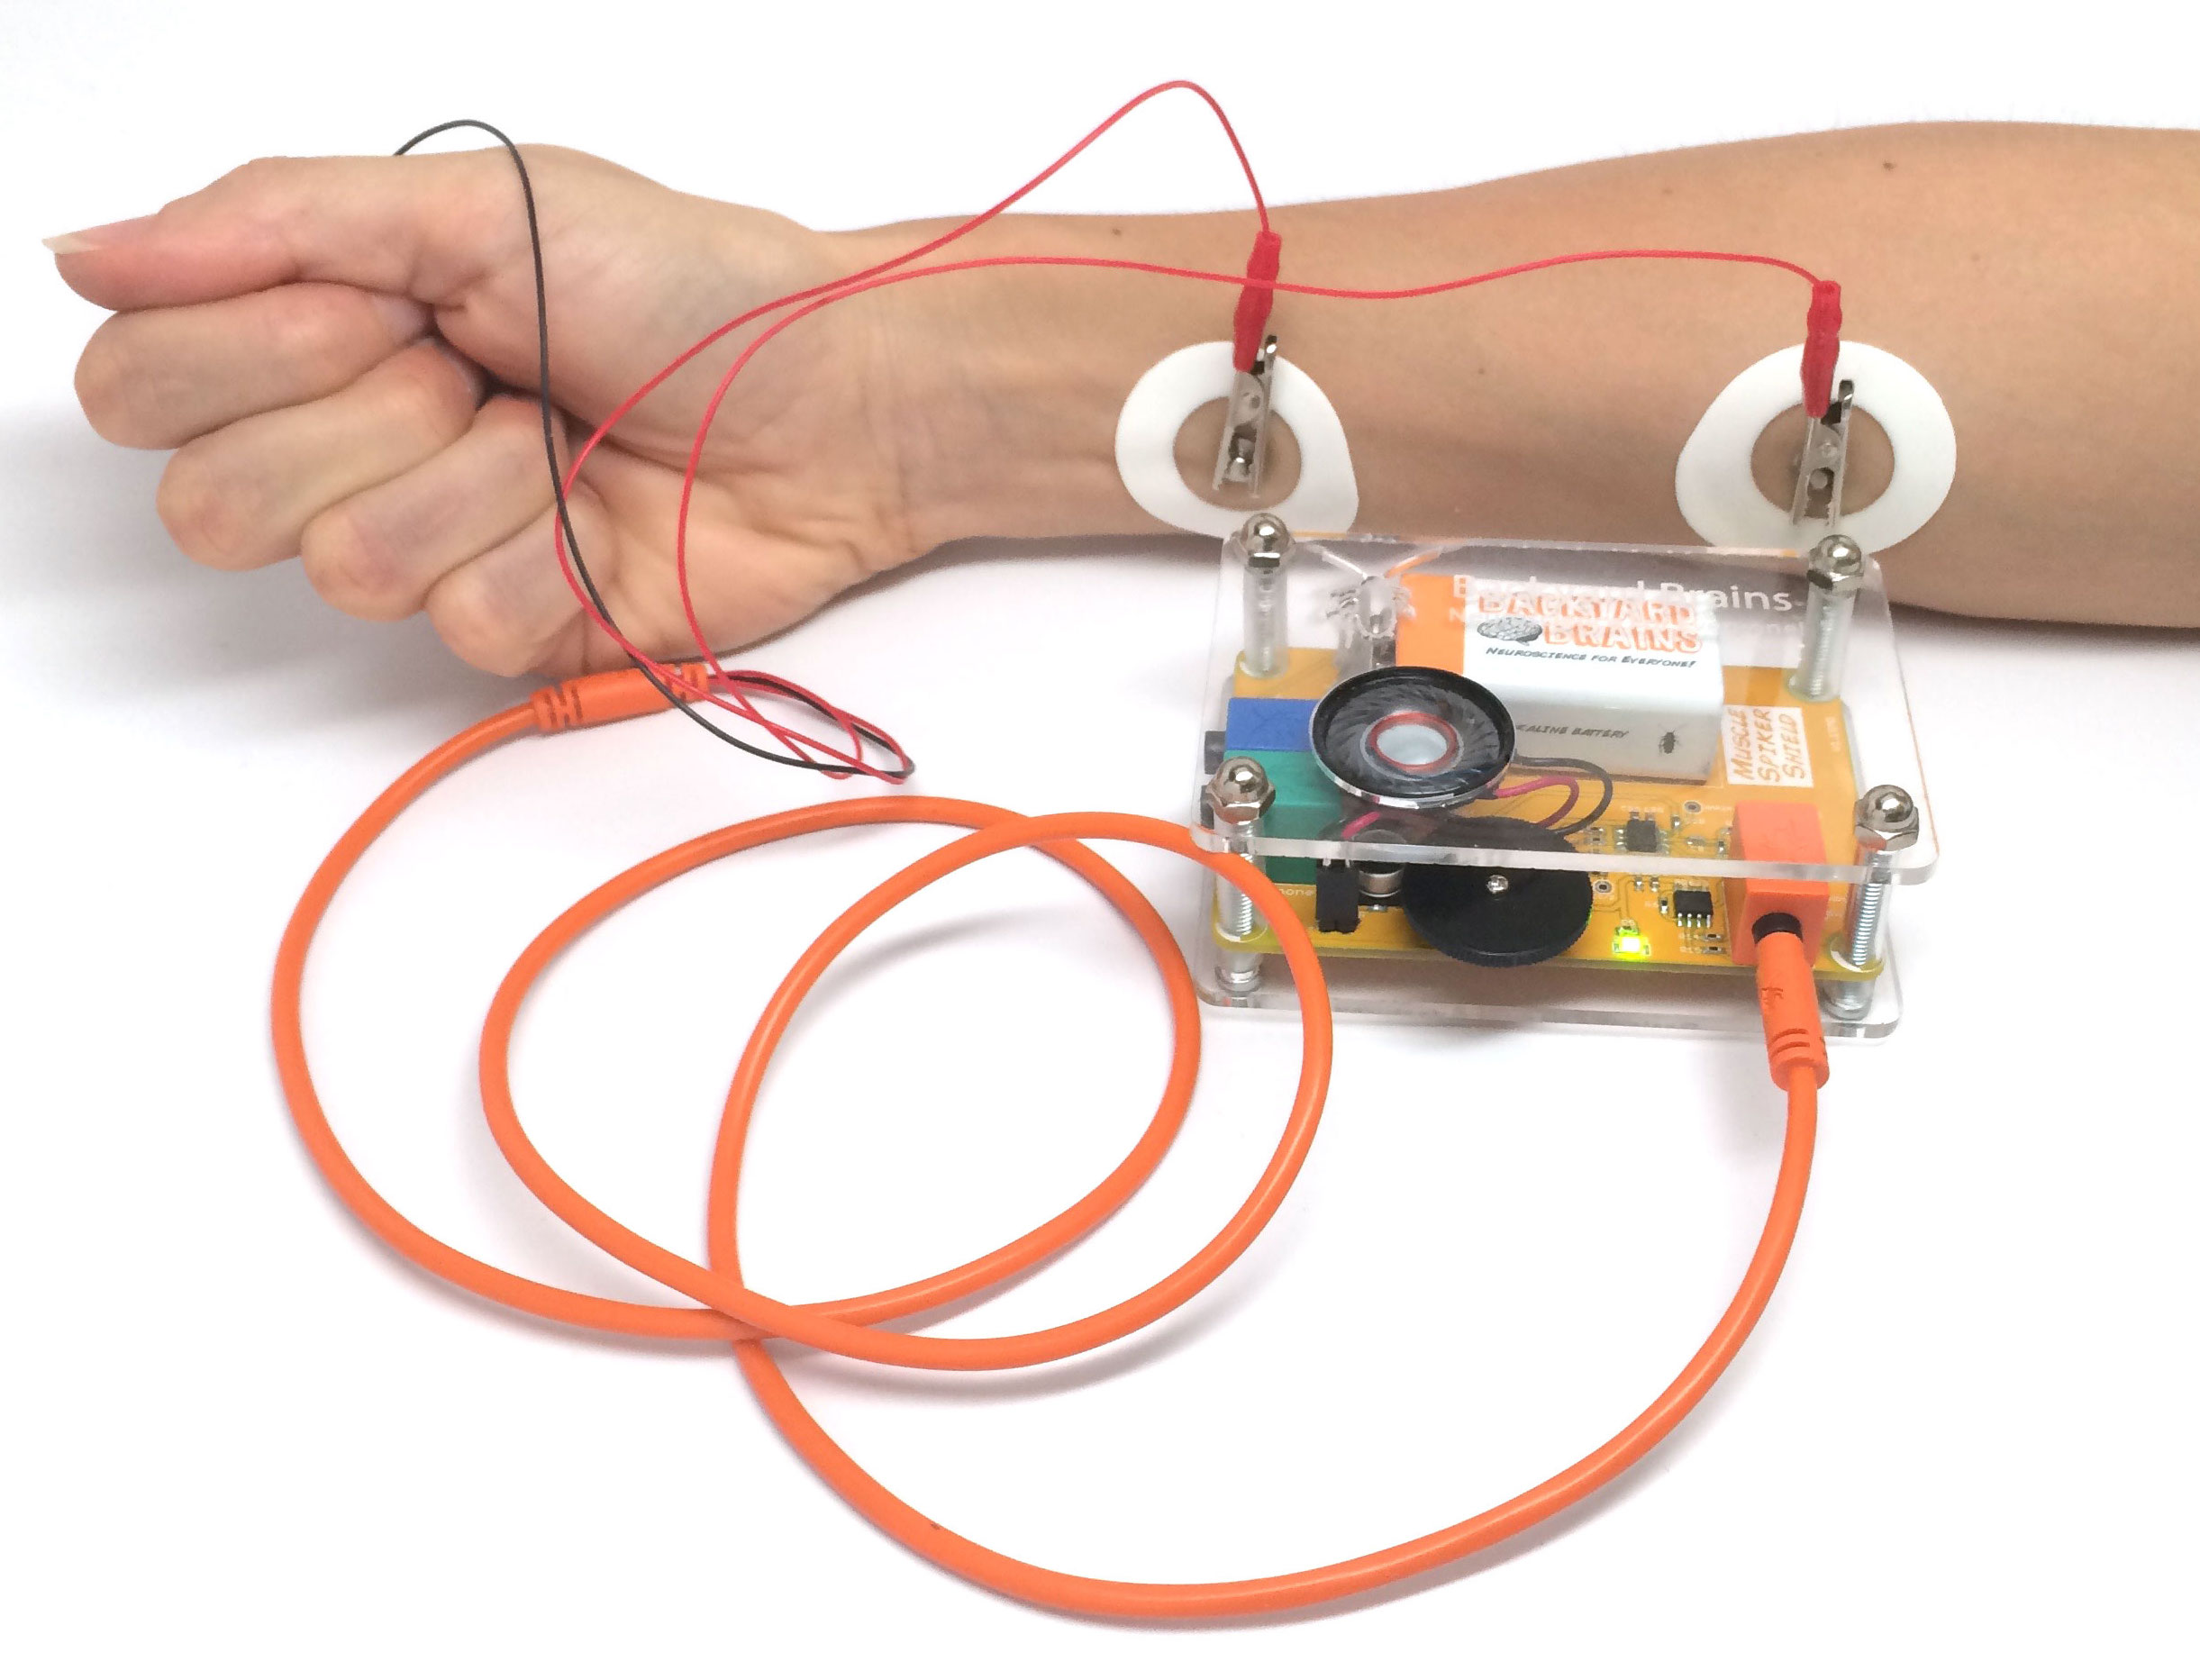
\includegraphics[width=0.8\textwidth]{figures/muscleSpikerBox.jpg}
\caption{\textit{Left}: EMG setup with electrodes connected to Muscle SpikerBox. (Connection to computer or smartphone not shown.) Image credit: Backyard Brains, CC BY SA.}
\label{fig:emgSetup}
\end{figure}

\item To improve the EMG signal, the area where the electrodes will be placed can be cleaned with alcohol prior to placement; wait until the area is dry to place the electrodes
\item Electrode gel can be placed to improve conduction but is often not necessary
\item To avoid noise artifacts, ensure that no clothing is touching the electrodes or brushing against the cables during recording
\end{enumerate}
 
\subsection*{2. Test EMG recordings}

\begin{enumerate}
\item Turn on the Muscle SpikerBox by rotating the black wheel switch on the side, a green light should turn on; note that electrodes should be connected before turning on the device and disconnected only after the device is turned off to avoid a nasty noise!
\item Open the Backyard Brains recording software and explore the controls and settings (for more info on software use, see \cite{spikeRecorder})

\begin{figure}[h!]
\centering
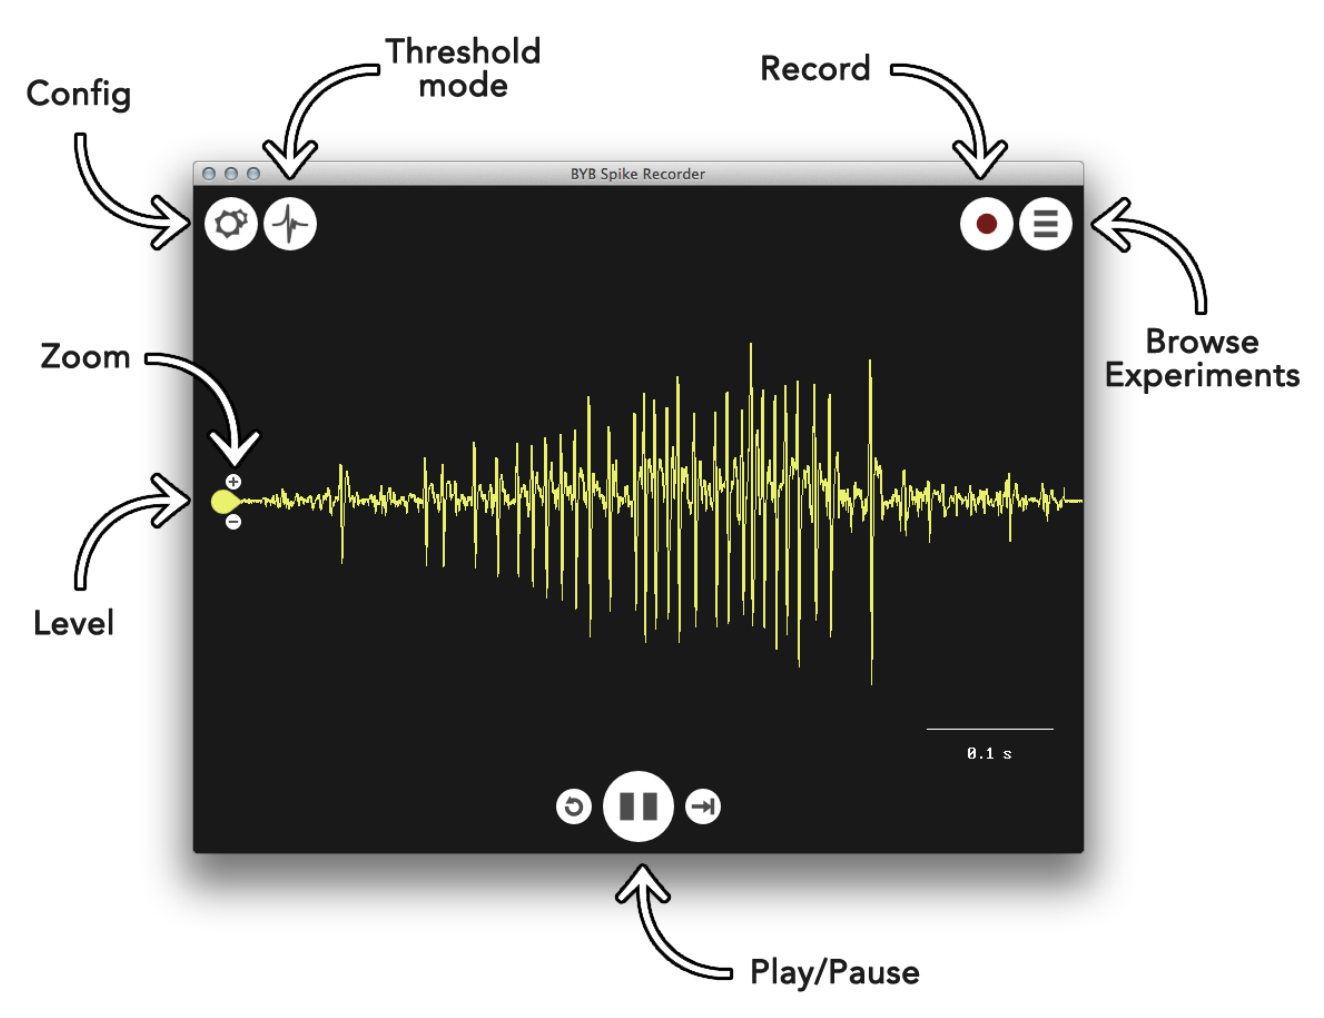
\includegraphics[width=0.8\textwidth]{figures/BBrecorder.png}
\caption{Recording software interface. Image credit: Backyard Brains, CC BY SA}
\label{fig:recorder}
\end{figure}

\item Snap your fingers near the recording device; if you see a corresponding artifact on the screen, this means you are recording only audio; to begin recording muscle activity, adjust the settings by pressing the `Config' button (Fig. \ref{fig:recorder}) (see \cite{spikeRecorder} for more details)
\item Ask the subject to briefly contract and relax the muscle of interest 
\item Verify that electric potentials are observed during the contraction; check your signal to noise rati; if the signal is too small, you can adjust the gain by turning the wheel switch to the right
\item Try saving a recording to your computer or smartphone (format will be .wav)
\end{enumerate}

\subsection*{3. Collect your data}

\begin{enumerate}
\item Make sure EMG is ready to record subject is in resting position
\item Before the recording begins, have the subject think about the type of movement they need to make to activate the muscle of interest, e.g., for the gastrocnemius muscle, this will involved standing on tip toes, whereas for the splenius capitis, this will involve lifting the head
\item When the subject is ready, press record on the Backyard Brains software interface
\item Instruct the subject to remain relaxed for 3-5 seconds after the recording begins, then contract the muscle of interest for 3-5 seconds, and then relax again for 3-5 seconds
\item Have the subject repeat the above sequence at least 3 times 
\item Terminate the recordings and save the data to your computer or smartphone
\item EMGs should be saved and exported in .wav format for analysis
\item Start a new recording to examine the effects of contraction force
\item Instruct the subject to perform the first contraction with very little force, then pause, then perform and second contraction with greater force, then pause, and finally perform a third contraction with maximal force
\item Terminate the recordings and save the data to your computer or smartphone
\item Start a new recording to examine fatigue
\item Instruct the subject to contract the muscle of interest and hold it for as long as they can; how long can they hold it? what happens as they start to tire? what happens if they use minimal versus maximum force?
\item Terminate the recordings and save the data to your computer or smartphone
\item Repeat steps 1-13 for each muscle belonging to the three lever systems types; subjects should rest for a few minutes between recording sessions
\item Remember to label your data so you know to which subject, muscle, and experiment type each recording belongs
\end{enumerate}

\section*{ACKNOWLEDGMENTS}
This work was supported by UNAM-DGAPA-PAPIME PE213817 and PE213219.

% BIBLIOGRAPHY
\renewcommand\refname{REFERENCES}
\renewcommand{\markboth}[2]{}%
\begin{footnotesize}
\bibliography{EMG}
\end{footnotesize}

\end{document}
